\documentclass[review]{elsarticle}
\usepackage{hyperref}
\usepackage[margin=1in]{geometry}
\usepackage{graphicx}
\usepackage{amsmath}
\usepackage{placeins}
\usepackage{comment}
\usepackage{gensymb}
\usepackage{lineno}
\usepackage{flexisym}
\usepackage{color}
\usepackage[title]{appendix}

\journal{Journal of Nuclear Materials}
\bibliographystyle{elsarticle-num}

\begin{document}

\begin{frontmatter}
\title{khadija paper on $\alpha$-U}

\author[ncsu,inl]{Benjamin Beeler\corref{qwe}}
\cortext[qwe]{Corresponding author}
\ead{bwbeeler@ncsu.edu}
\author[lanl]{David Andersson}
\author[inl]{Chao Jiang}
\author[wisc,inl]{Yongfeng Zhang}
\address[ncsu]{North Carolina State University, Raleigh, NC 27607}
\address[inl]{Idaho National Laboratory, Idaho Falls, ID 83415}
\address[lanl]{Los Alamos National Laboratory, Los Alamos, NM 87545}
\address[wisc]{University of Wisconsin-Madison, Madison, WI 53706}

\begin{abstract}



\end{abstract}
\end{frontmatter}

\section{Introduction}



\section{Computational Details}

The Large-scale Molecular Massively Parallel Simulator (LAMMPS) \cite{plimpton1995} is utilized to perform molecular dynamics (MD) simulations. 

In fig. \ref{fig:1} there is an example figure. 

\begin{figure}[h]
 \centering
 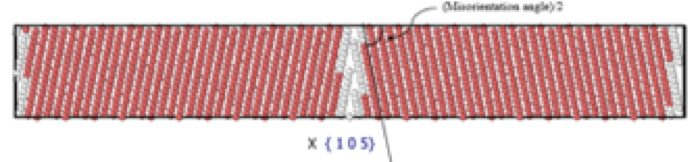
\includegraphics[width=0.95\textwidth]{fig_ex.png} 
 \caption{An example }
 \label{fig:1}
\end{figure}

\FloatBarrier

The formation energy of point defects is calculated via equation \ref{eq:eform}: 

\begin{equation}
\label{eq:eform}
E_f = E^* - \frac{n \pm 1}{n} \times E_0
\end{equation}

where E$^{*}$ is the energy of a system with a defect (with n $\pm 1$ atoms), \textit{n} is the number of atoms in the defect-free system and E$_{0}$ is the energy of a defect-free system with \textit{n} atoms. Equation \ref{eq:eform} utilizes (\textit{n} + 1) for interstitials and (\textit{n} - 1) for vacancies. 

\section{Results}
\subsection{Dummy title}


\FloatBarrier

\section{Conclusions}



\section{Acknowledgement}
This will change and we will make sure we have the right one.

This work is supported by the U.S. Department of Energy, Office of Nuclear Energy, Nuclear Energy Advanced Modeling and Simulation (NEAMS) Program. This manuscript has been authored by Battelle Energy Alliance, LLC under Contract No. DEAC07-05ID14517 with the U.S. Department of Energy. The United States Government retains and the publisher, by accepting the article for publication, acknowledges that the United States Government retains a nonexclusive, paid-up, irrevocable, world-wide license to publish or reproduce the published form of this manuscript, or allow others to do so, for United States Government purposes.  Los Alamos National Laboratory, an affirmative action/equal opportunity employer, is operated by Los Alamos National Security, LLC, for the National Nuclear Security Administration of the U.S. Department of Energy under Contract No. DE-AC52-06NA25396.  This research made use of the resources of the High Performance Computing Center at Idaho National Laboratory, which is supported by the Office of Nuclear Energy of the U.S. Department of Energy and the Nuclear Science User Facilities under Contract No. DE-AC07-05ID14517.



\bibliography{MARMOTbib}

\end{document} 
